\chapter{Interrogazione dell'ontologia}

\section{SWRL}
Per permettere al reasoner di inferire maggiori informazioni riguardanti l'ontologia sono state realizzate alcune regole SWRL.

Le seguenti regole sono state realizzate per permettere al reasoner di inferire il valore di energia che una batteria può effettivamente assorbire o immettere.

Siccome varie sono le casistiche da controllare, sono state create quattro regole per i calcoli inerenti.\\


[\ref*{fig:bothlessorequal}] \texttt{Capacità massima di carica <= Capacità di carica e\\
    Capacità massima di scarica <= Capacità di scarica}

\begin{figure}[H]
    \centering
    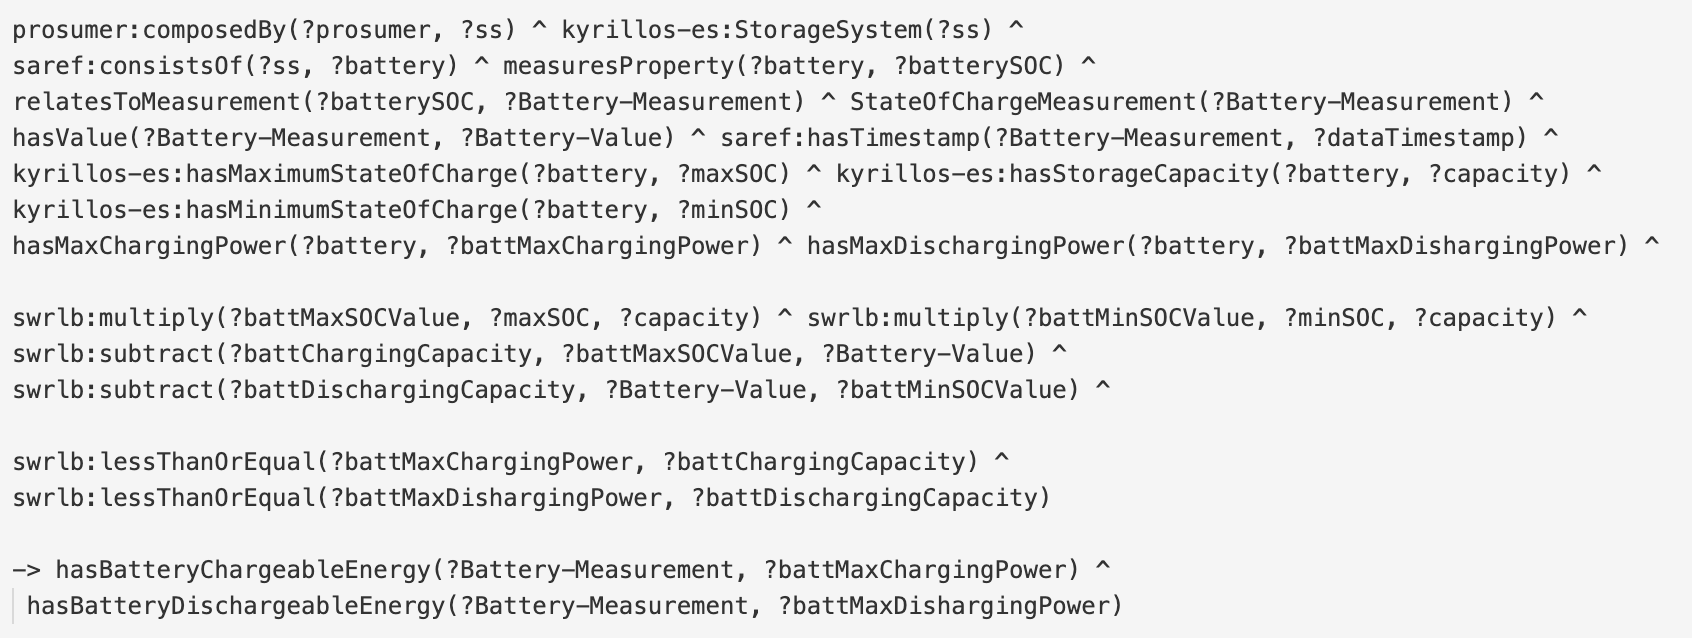
\includegraphics[width=15cm]{images/both <=.png}
    \caption{Screenshot della prima regola.}
    \label{fig:bothlessorequal}
\end{figure}

[\ref*{fig:charginglessorequal}] \texttt{Capacità massima di carica <= Capacità di carica e\\ Capacità massima di scarica > Capacità di scarica}

\begin{figure}[H]
    \centering
    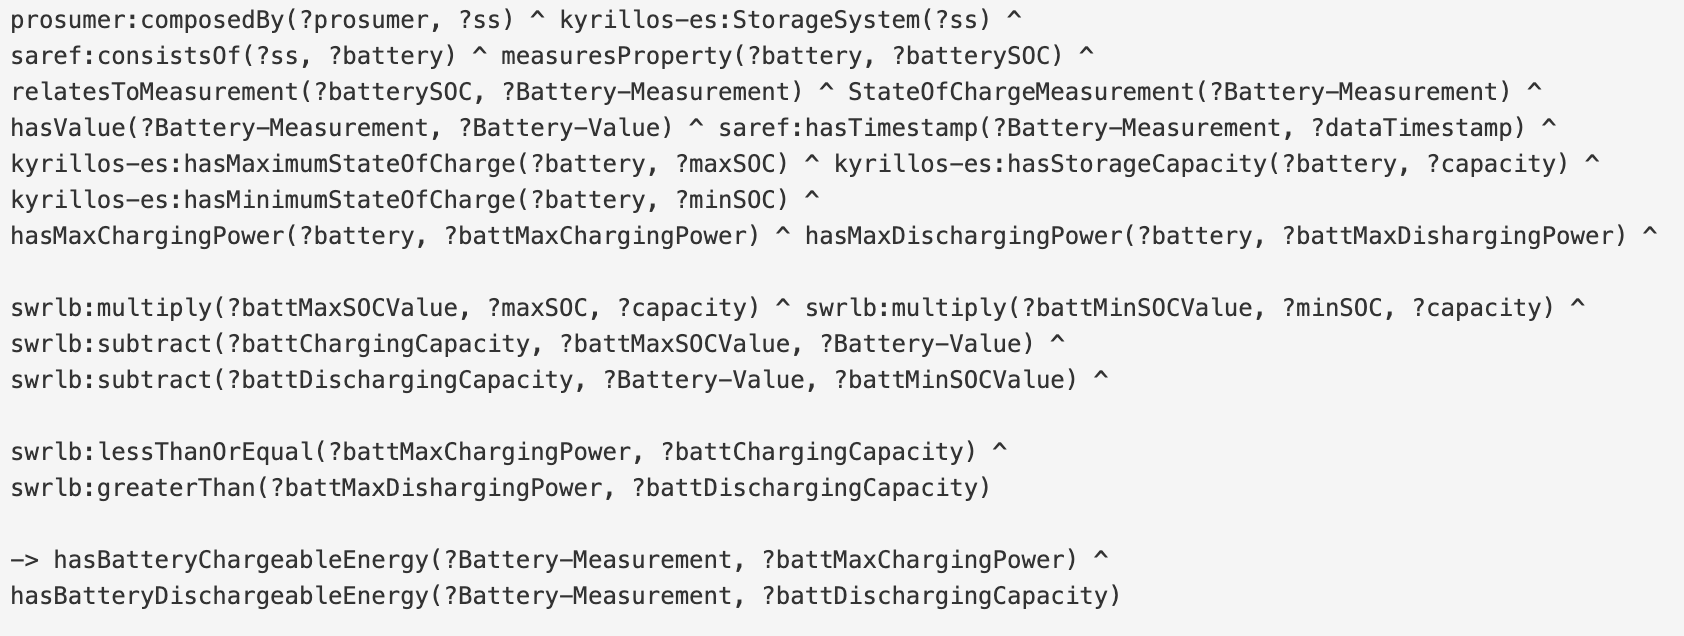
\includegraphics[width=15cm]{images/charging <=.png}
    \caption{Screenshot della seconda regola.}
    \label{fig:charginglessorequal}
\end{figure}

[\ref*{fig:charginggreater}] \texttt{Capacità massima di carica > Capacità di carica e\\ Capacità massima di scarica <= Capacità di scarica}

\begin{figure}[H]
    \centering
    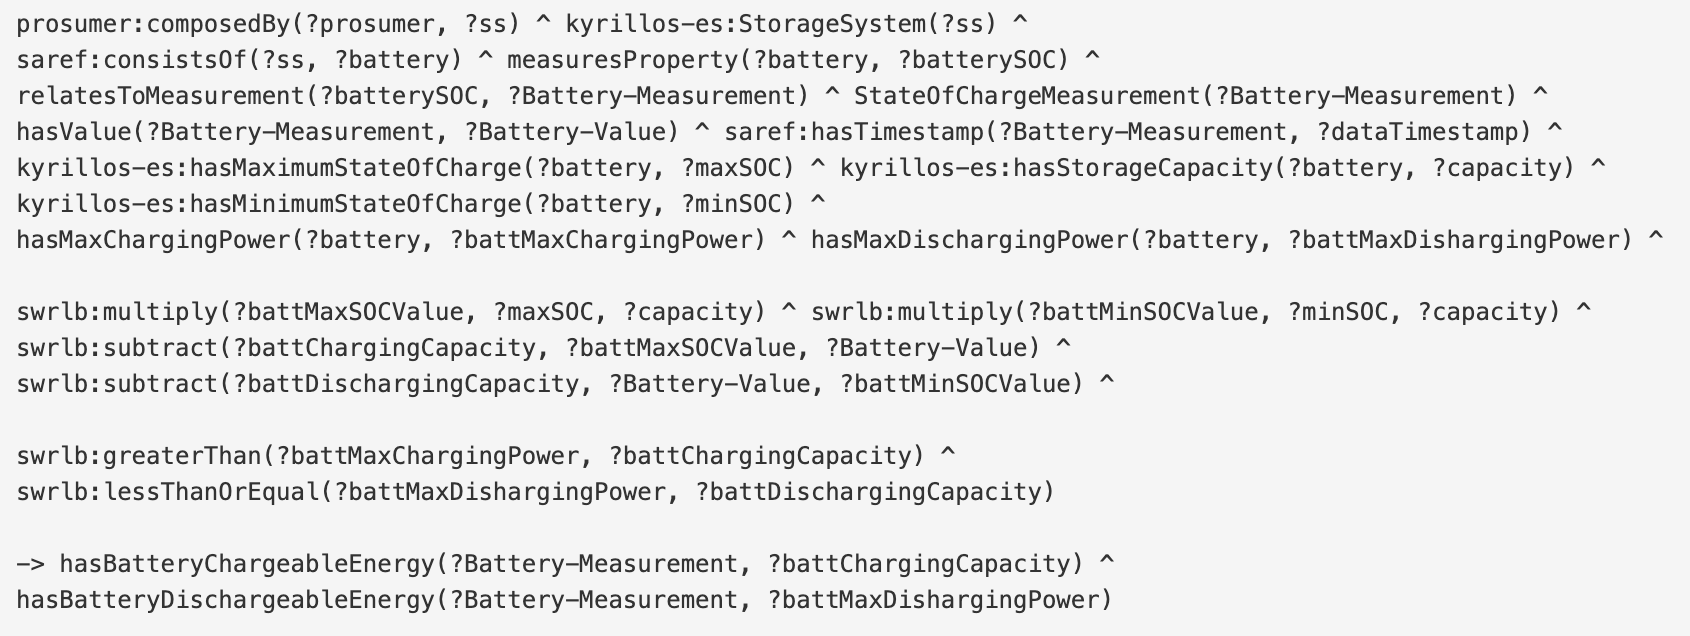
\includegraphics[width=15cm]{images/charging >.png}
    \caption{Screenshot della terza regola.}
    \label{fig:charginggreater}
\end{figure}

[\ref*{fig:bothgreater}] \texttt{Capacità massima di carica > Capacità di carica e\\ Capacità massima di scarica > Capacità di scarica}

\begin{figure}[H]
    \centering
    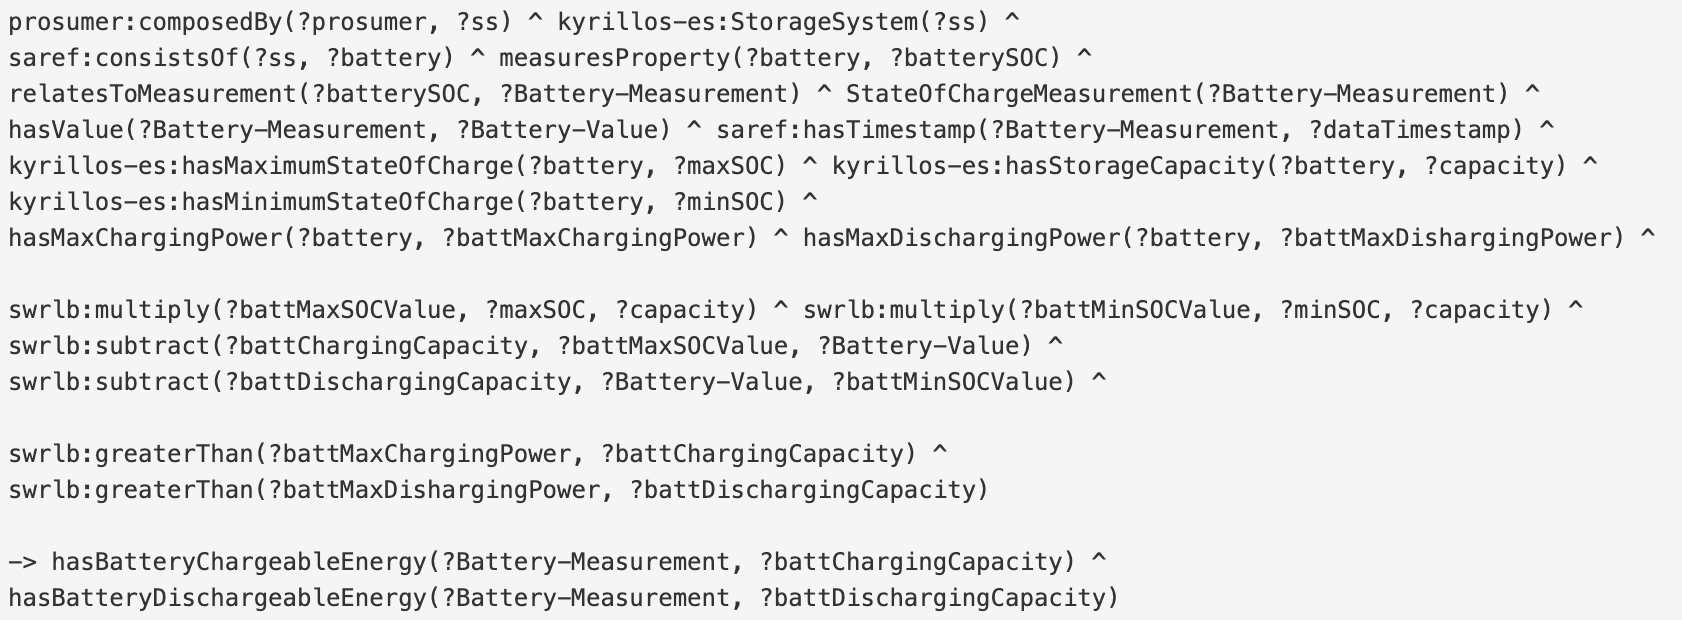
\includegraphics[width=15cm]{images/both >.png}
    \caption{Screenshot della quarta regola.}
    \label{fig:bothgreater}
\end{figure}

\section{SPARQL}

\subsection{PREFIX}
Per leggibilità i prefissi utilizzati per le query SPARQL verranno visionati solamente in questa sezione.

\begin{figure}[H]
    \centering
    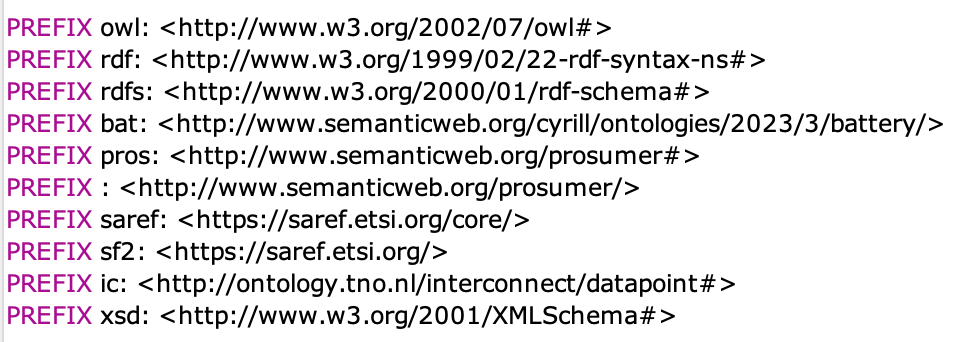
\includegraphics[width=15cm]{images/prefissi.png}
    \caption{Prefissi da anteporre alle query sull'ontologia.}
    \label{fig:prefix}
\end{figure}

\subsection{Query che calcola l'energia che può fornire o assorbire uno Storage System}

\begin{figure}[H]
    \centering
    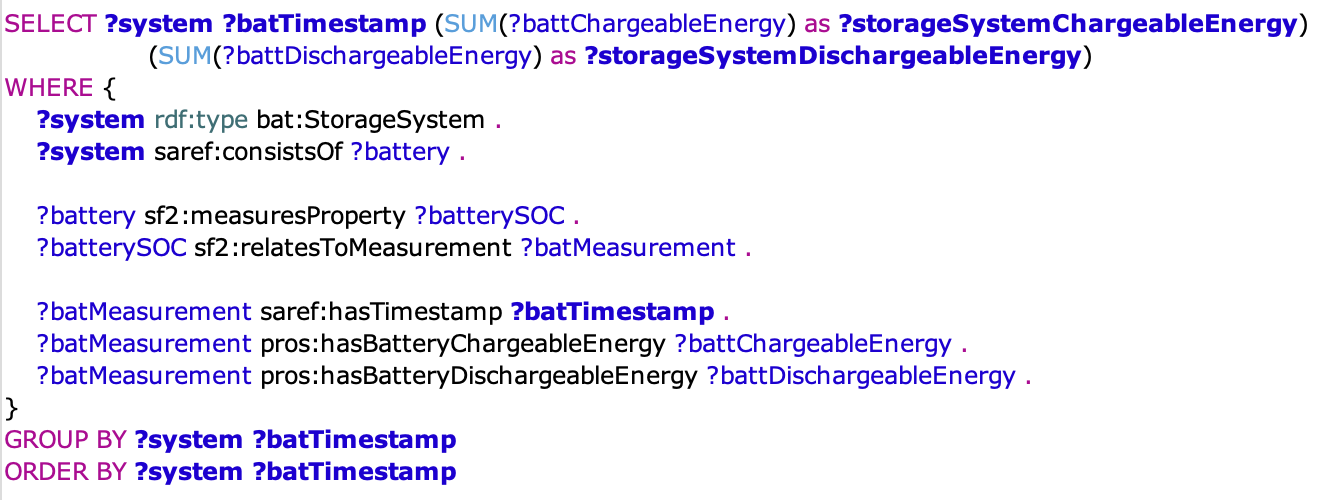
\includegraphics[width=15cm]{images/subquery.png}
    \caption{Query per il calcolo dell'energia che uno Storage System può assorbire o fornire.}
    \label{fig:subquery}
\end{figure}

\begin{figure}[H]
    \centering
    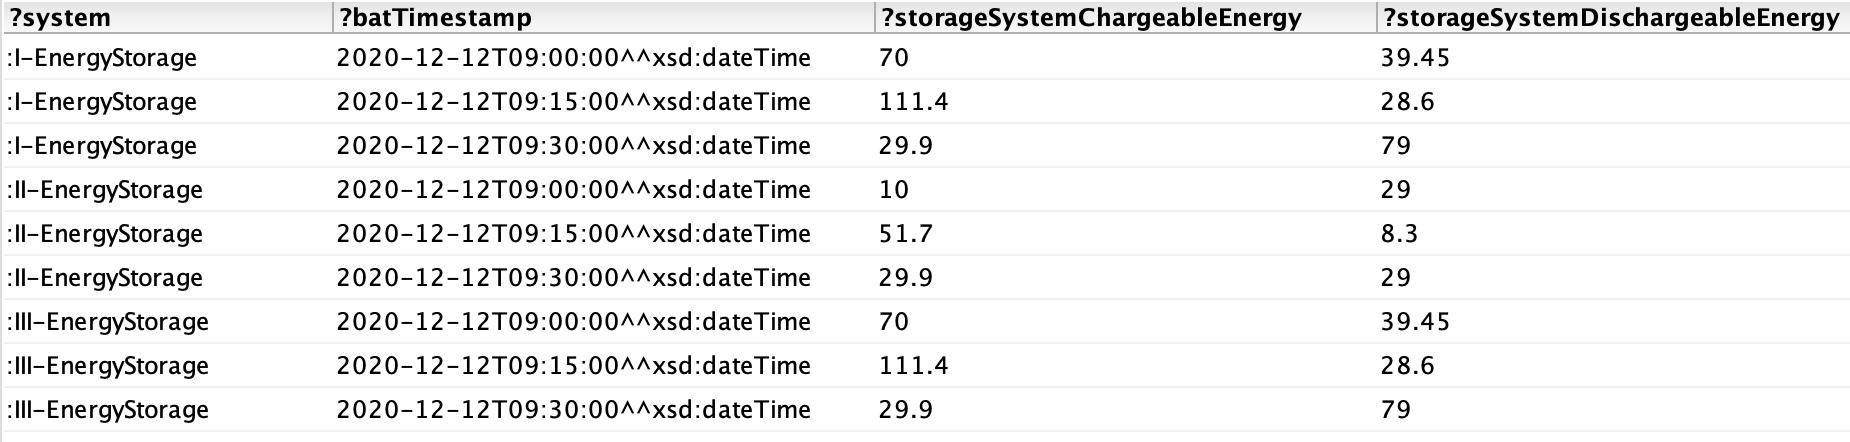
\includegraphics[width=15cm]{images/subquery_res.png}
    \caption{Risultati della query per il calcolo dell'energia che uno Storage System può assorbire o fornire.}
    \label{fig:subquery_res}
\end{figure}

\subsection{Query sul calcolo della flessibilità del contatore M1}

\subsection{Query per il calcolo di M1 e M2 in prosumer di configurazione 1 e 2}

\subsection{Query per il calcolo di M1, M2 e M3 in prosumer di configurazione 3}